\documentclass[11 pt]{article}
\pagenumbering{gobble}
\usepackage[bmargin=1in,tmargin=1in,lmargin=1.0in,rmargin=1.0in]{geometry}
\usepackage[dvipsnames]{xcolor}
\usepackage{amsfonts,amsmath,color,amssymb, url, enumerate, bbm}
\usepackage{pgfplotstable, pgfplots}
\usepackage{graphicx}
\usepackage{tikz}
\usepackage[title,titletoc]{appendix}
\usetikzlibrary{patterns, arrows}
\usepackage{subcaption}
\usepackage[noend]{algpseudocode}
\usepackage{algorithm}
\usepackage{float}
\usepackage{dashbox}
\pgfplotsset{compat=newest}
\usepackage{multicol}
\usepackage{hyperref}
\hypersetup{
    colorlinks=true,
    linkcolor=blue,
    filecolor=magenta,      
    urlcolor=blue,
}

\newtheorem{thm}{Theorem}[section]
\newtheorem{lm}{Lemma}[section]
\newtheorem{pf}{Proof}[section]
\newtheorem{defn}{Definition}[section]

\newcommand{\mcom}[1]{\marginpar{#1}}
\newcommand{\ilcom}[1]{\textcolor{red}{[#1]}}   
\newcommand{\dbbox}[1]{\dashbox{\textbf{#1}}}          

\title{ENGRI 1101 Software Installation}
\date{}

\usepackage{setspace}
\singlespacing
\begin{document}

\maketitle

\section{Anaconda Installation}

In this class, we will use a Python distribution called \href{https://www.anaconda.com/}{Anaconda}. More specifically, we will use the Individual Edition. First, download the \href{https://www.anaconda.com/products/individual}{Anaconda Graphical Installer}. Over the course of the semester, you will complete some labs in Jupyter Notebooks which allow you to run Python code. Many of these labs rely on various Python packages. A Python package is essentially pre-bundled code that serves some functionality. You will need to install the following packages. 

\begin{center}
\begin{tabular}{ll}
 \texttt{gilp} & Visualize the simplex algorithm and solve linear programs \\
 \texttt{ortools} & Google's optimization suite \\
 \texttt{networkx} &  Create and manipulate complex networks \\
 \texttt{matplotlib} & Publication quality figures in python \\
 \texttt{pandas} & High-performance, easy-to-use data structures and data analysis tools \\
 \texttt{bokeh} & Statistical and novel interactive html plots for python \\
 \texttt{shapely} & Manipulation and analysis of geometric objects in the cartesian plane \\
 \texttt{scipy} & Scientific library for python \\
 \texttt{scikit-image} & Image processing routines for scipy \\
 \texttt{numpy} & Array processing for numbers, strings, records, and objects \\
\end{tabular}
\end{center}

\noindent \textbf{Note:} If you are using Windows, you must download the following software first: \href{https://visualstudio.microsoft.com/downloads/?q=Visual+C\%2B\%2B+Redistributable+for+Visual+Studio}{Microsoft Visual C++ Redistributable for Visual Studio 2019} (select the x64 version at the bottom of the page). This is because the OR-Tools library for Python is a wrapper for the C++ native library. \newline

\begin{center}
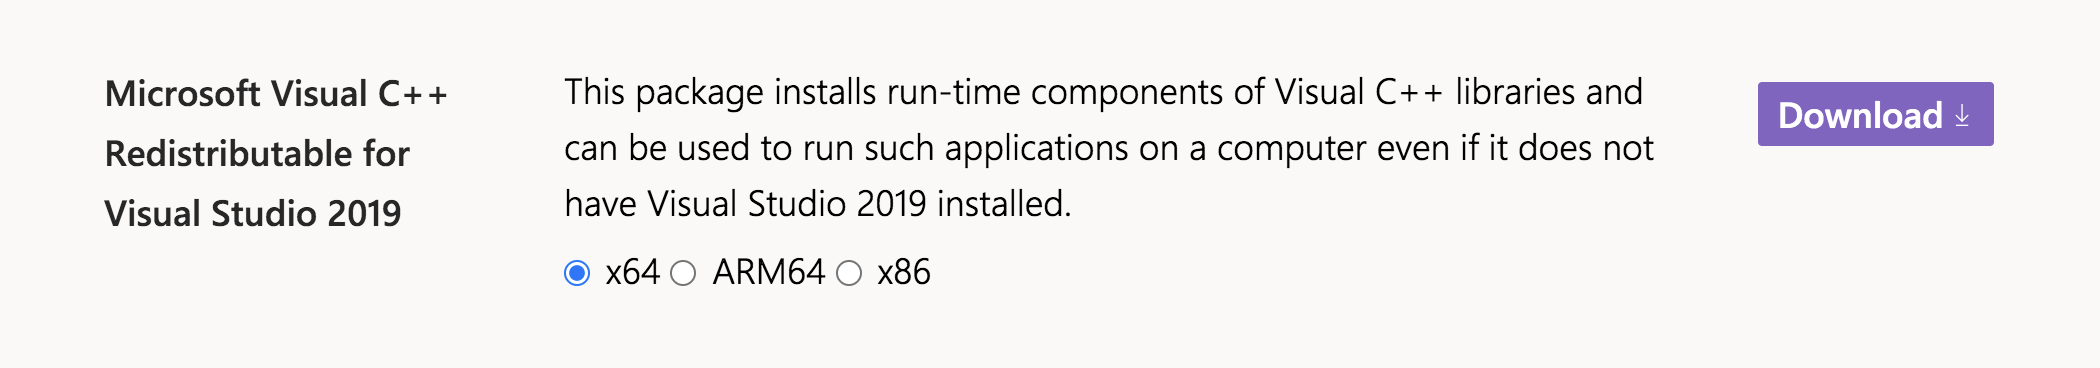
\includegraphics[scale=0.4]{vs_download}
\end{center}

We will now walk through the steps for creating a virtual environment in Anaconda. In a virtual environment, the installed packages are isolated to that environment. Hence, if you install a python package in one environment, you could not reference it in another. You will import an environment that already has all necessary packages installed. First, open up the Anaconda application.

\begin{enumerate}

\item Navigate to the \texttt{Environments} tab
\item Click \texttt{Import}. You will get a pop-up like the one below. Name your environment \texttt{engri\char`_1101}. For the specification file, select \texttt{engri\char`_1101.yml} which has been distributed to you. 

\begin{center}
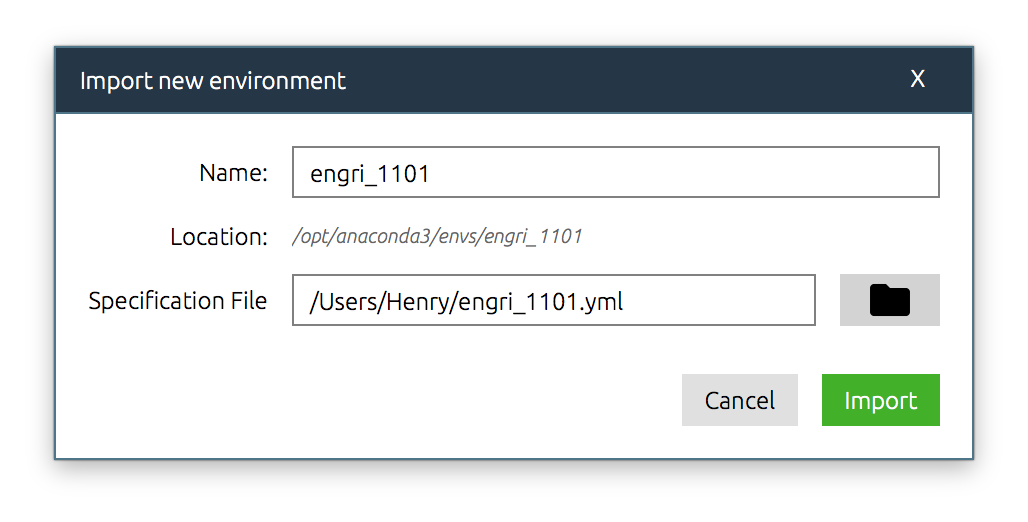
\includegraphics[scale=0.4]{import_env}
\end{center}

\item Once the installation is complete, you should see \texttt{engri\char`_1101} in your list of environments. Navigate back to the \texttt{Home} tab. Change the \texttt{Applications on} drop-down to your new \texttt{engri\char`_1101} environment.

\begin{center}
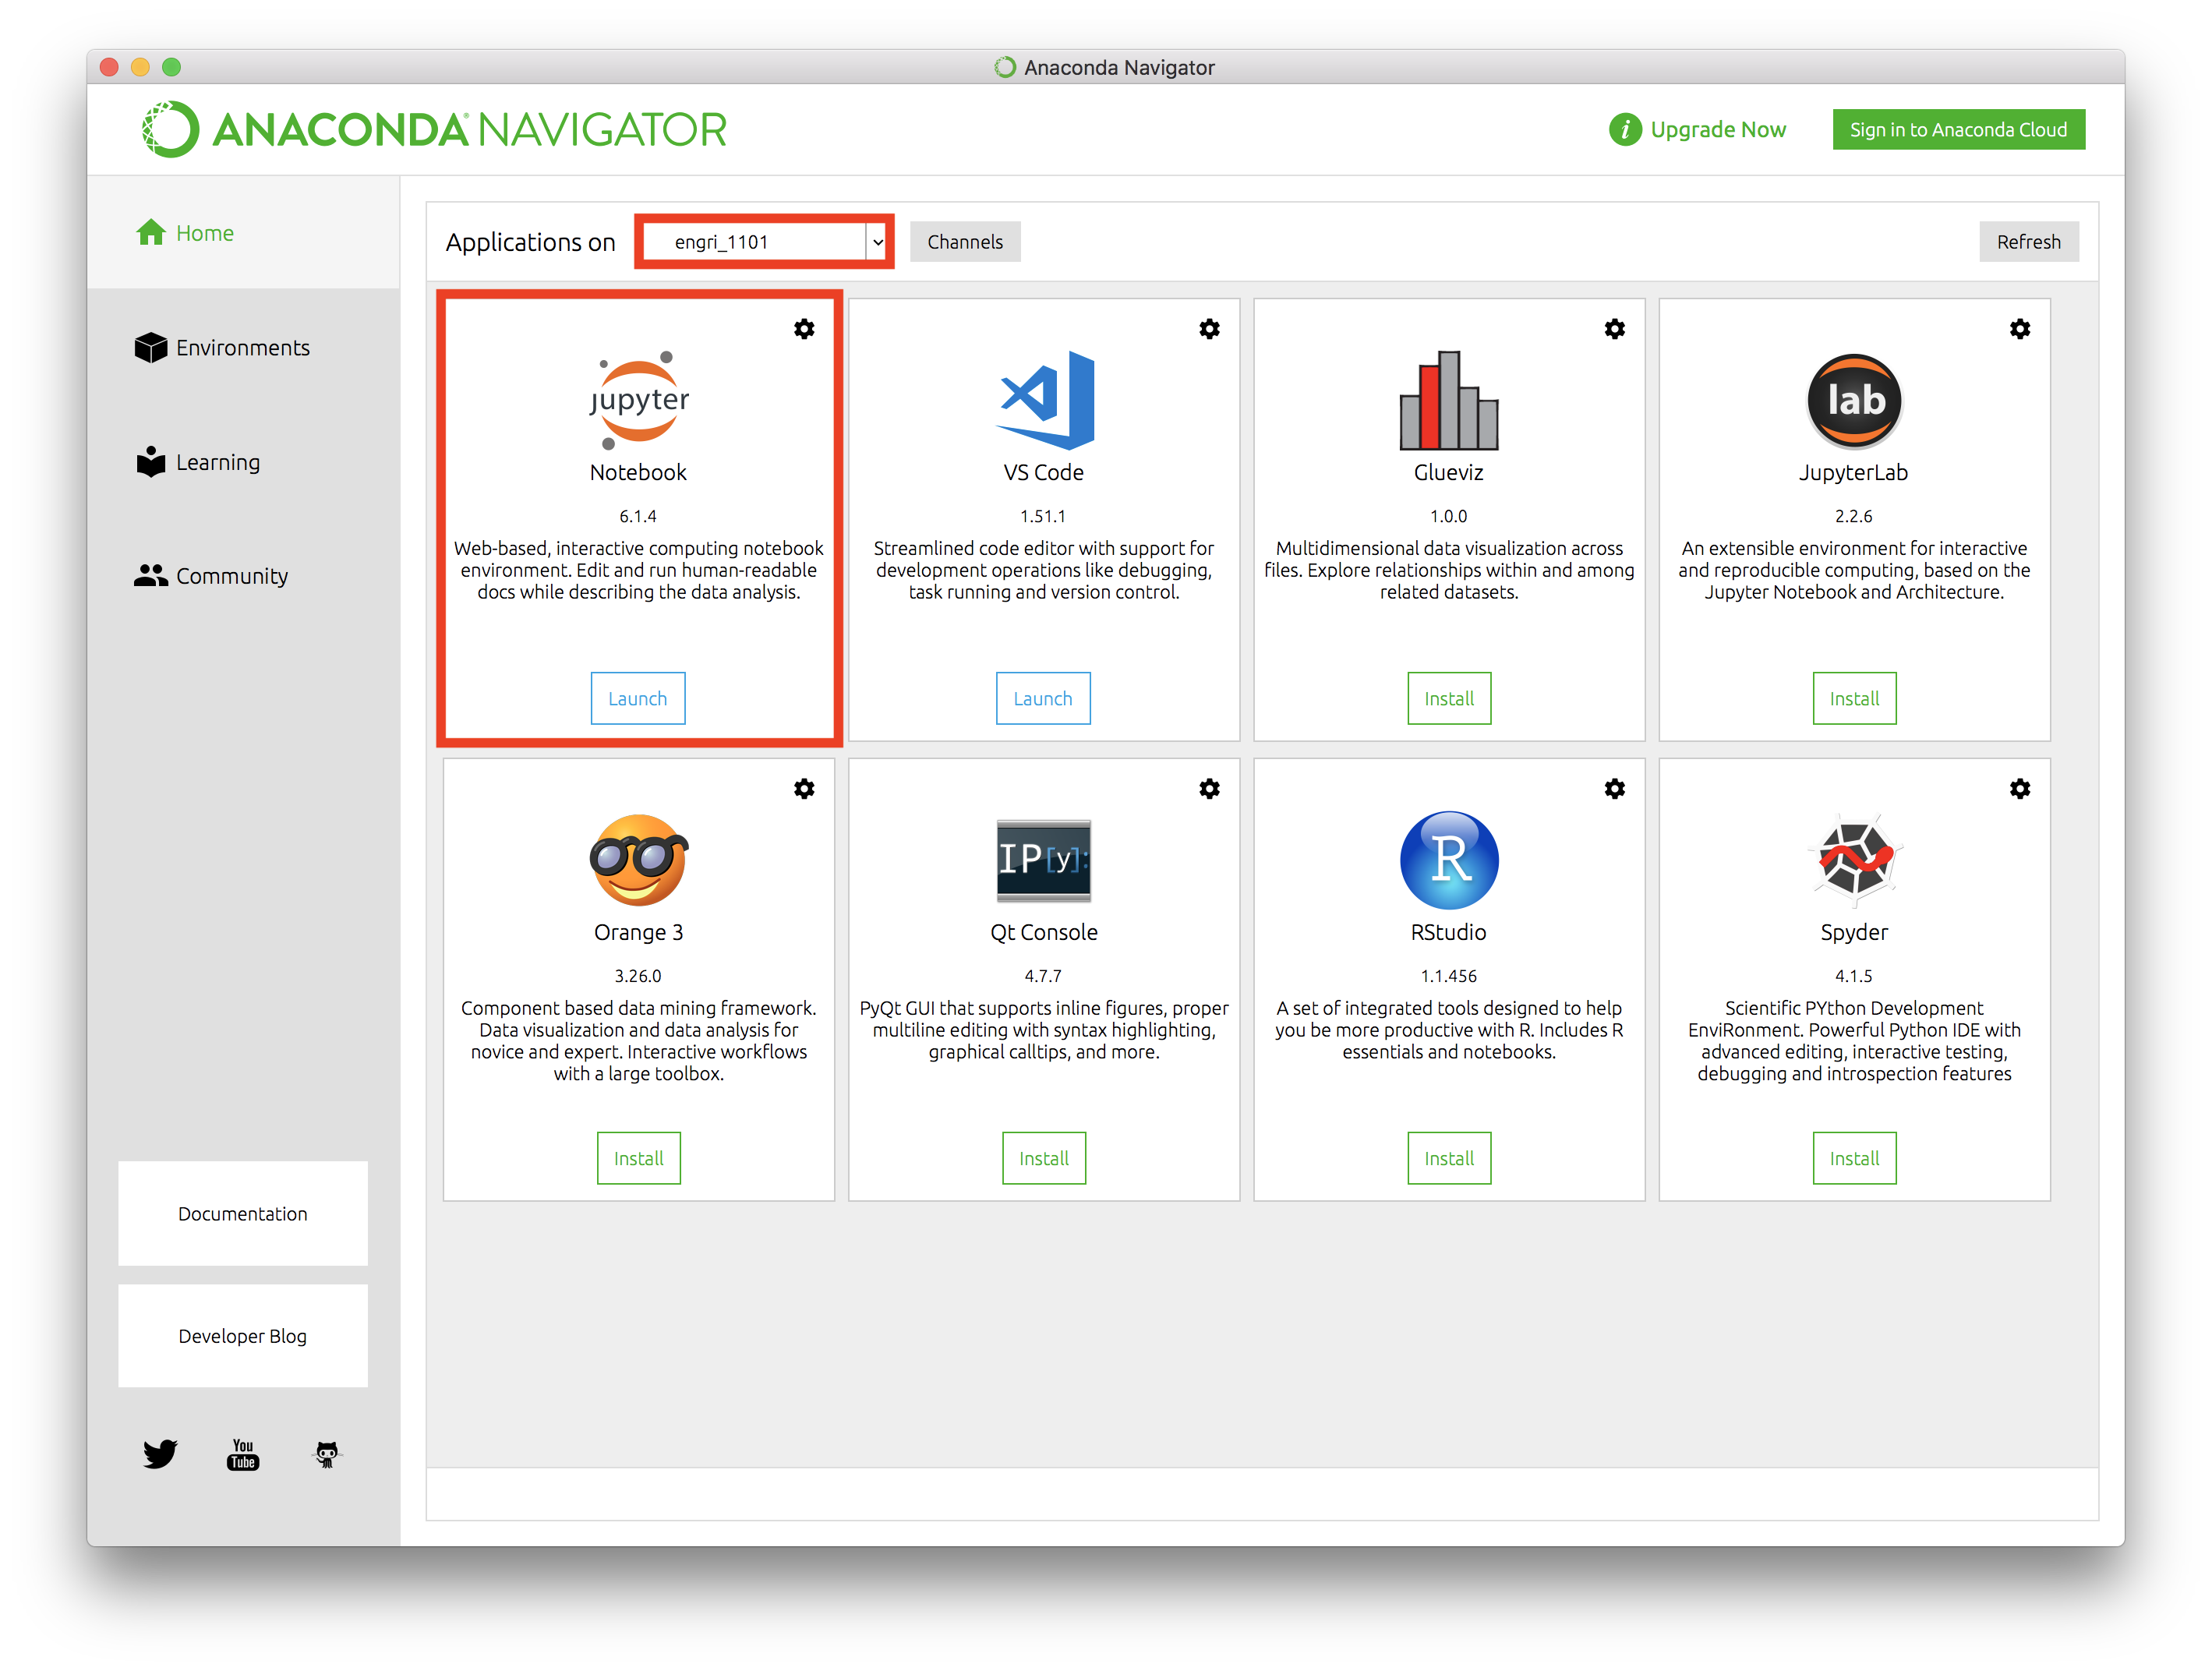
\includegraphics[scale=0.3]{home_tab}
\end{center}

\item Launch the \texttt{Jupyter Notebook} application which will open up a web-browser tab displaying the home directory of your system. 

\item Navigate to the file \texttt{test\char`_install.ipynb} and open it. Run the first block of code. This should run without errors if your virtual environment has been set up properly!

\end{enumerate}

\newpage

\section{Gurobi Installation}

The Python package \texttt{ortools} is Google's optimization suite. It contains an open-source linear program (LP) and integer linear program (ILP) solver. However, it can also serve as a way to interact with the cutting-edge Gurobi solver. In order to solve LPs and ILPs in \texttt{ortools} using Gurobi, you will need to download additional software. First, you will create an \href{https://pages.gurobi.com/registration}{Academic User Account}. Next, download the \texttt{Gurobi Optimizer} found at \href{https://www.gurobi.com/downloads/}{Gurobi Downloads}. Lastly, you will need to create an academic license to use the software. Register for an \href{https://www.gurobi.com/downloads/end-user-license-agreement-academic/}{Academic License}. After generating your unique academic license, you will be given a line to run in your terminal. When prompted, select the default location for the license file.


\begin{center}
%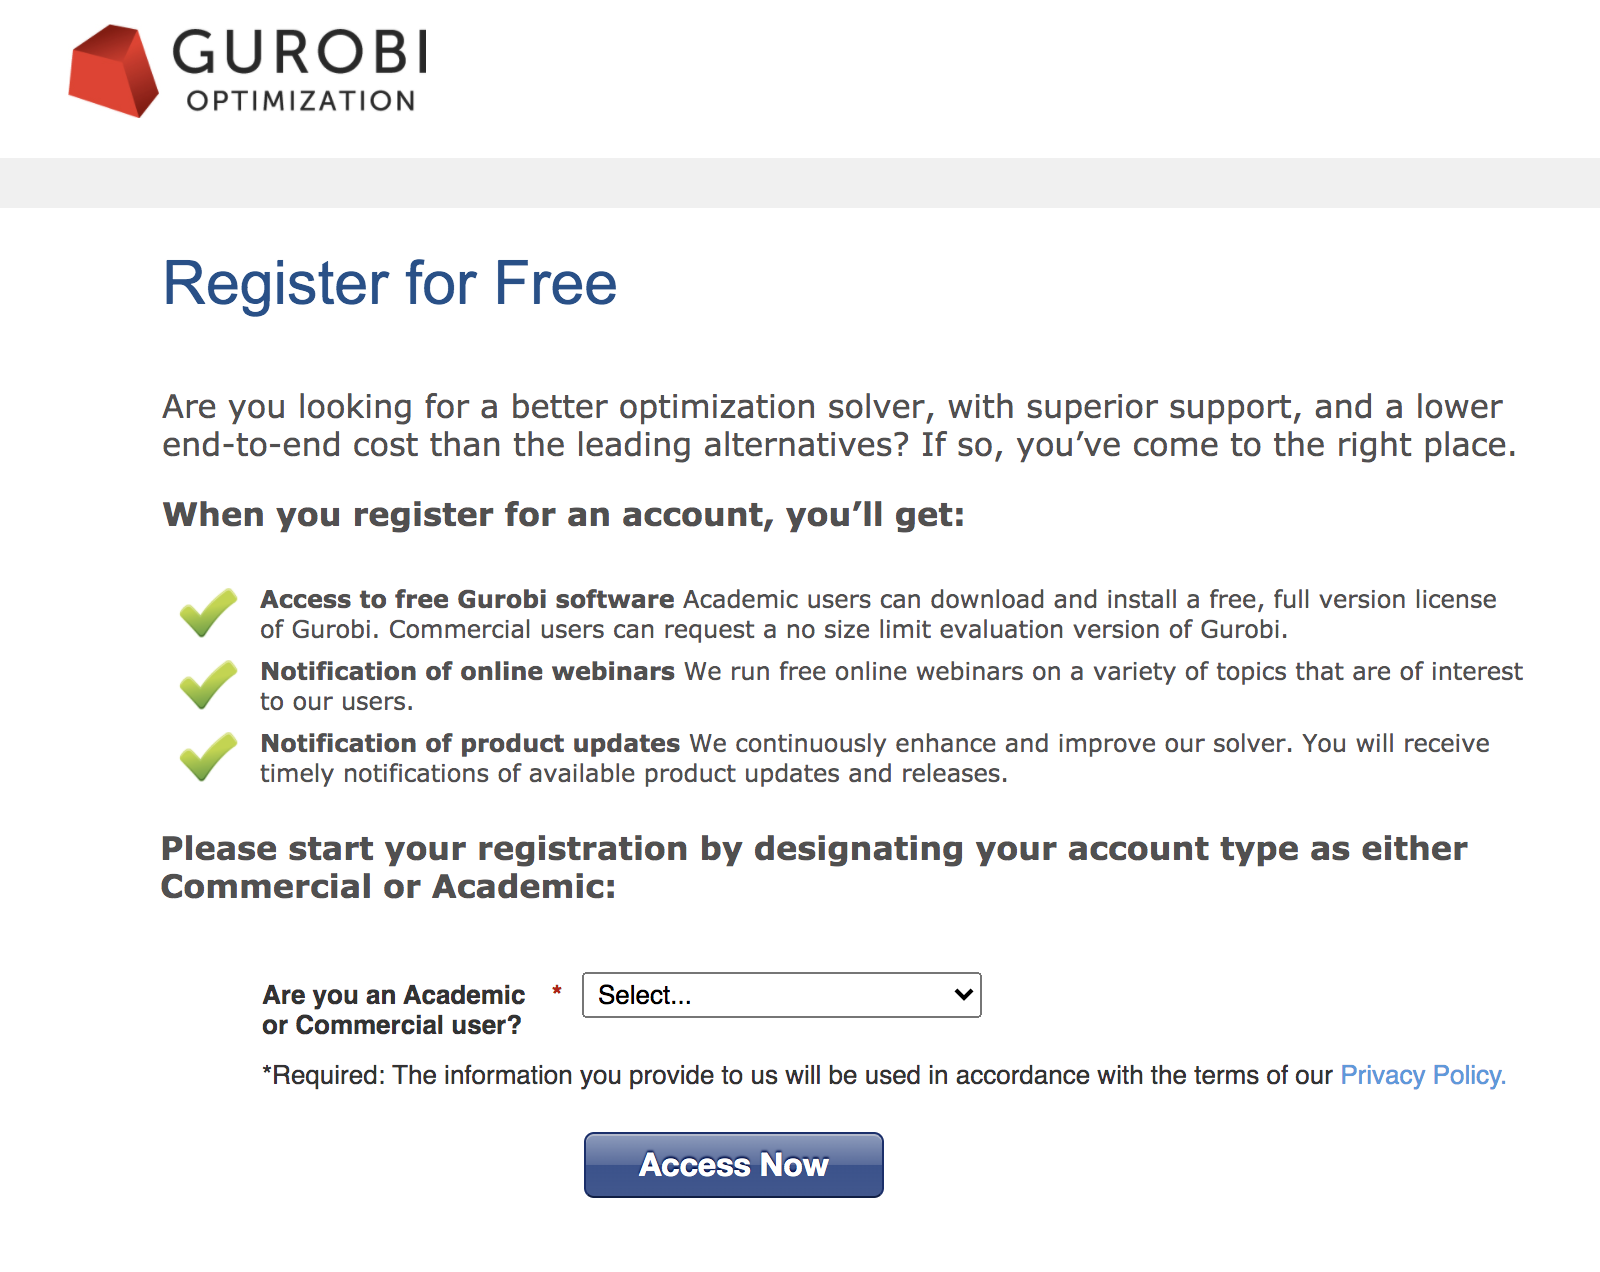
\includegraphics[scale=0.3]{gurobi_registration}
\end{center}
\begin{center}
%
\includegraphics[scale=0.3]{gurobi_download}
\end{center}


\end{document}